\documentclass[11pt,a4paper]{article}
\usepackage[margin=2cm]{geometry}
\usepackage[T1]{fontenc}
\usepackage{lmodern}
\usepackage{graphicx}
\usepackage{booktabs}
\usepackage{makecell}
\usepackage{subcaption}
\usepackage{amsmath}
\usepackage[hidelinks]{hyperref}
\usepackage{xcolor}
\graphicspath{{VR564554_image_Classification/results/}}

\newcommand{\authorname}{Tommaso Bell\`e}
\newcommand{\studentid}{VR564554}

\title{Homework 2: Transfer Learning for Fine-Grained Pet Breed Classification\\
\large Computer Vision -- Fall 2026}
\author{\authorname\ (\studentid)}
\date{}
\setlength{\textfloatsep}{10pt plus 2pt minus 2pt}

\begin{document}
\maketitle

\noindent\textbf{GitHub repository (code, splits, metrics, figures and checkpoints):}\\
\url{https://github.com/ILDucaJr/VR564554_image_Class}

\section{Introduction}
We compare three ways of adapting an ImageNet-pre-trained MobileNetV3-Small~\cite{mobilenetv3}
to the 37-class breed classification task of the Oxford-IIIT Pet dataset~\cite{pets}:
(1)~full fine-tuning, (2)~training only the fully connected classifier head on a frozen
feature extractor, and (3)~extracting frozen features and training a scikit-learn
classifier~\cite{sklearn}. Data splits, preprocessing, architecture and evaluation are
identical for all approaches, and the test set is used once per selected model.

\section{Dataset and experimental protocol}
\paragraph{Data.} Oxford-IIIT Pet~\cite{pets} contains 7{,}349 images of 37 breeds
(12 cat and 25 dog breeds), released under the Creative Commons Attribution-ShareAlike~4.0
license and available at \url{https://www.robots.ox.ac.uk/~vgg/data/pets/}. Images are not
redistributed in the repository; they are downloaded automatically by
\texttt{torchvision.datasets.OxfordIIITPet}. We use the 37 breed labels, not the
cat/dog labels.

\paragraph{Splits.} We keep the official \texttt{trainval} (3{,}680 images) and \texttt{test}
(3{,}669 images) partitions. \texttt{trainval} is split 80/20 into training (2{,}944) and
validation (736) sets, stratified by breed (\texttt{train\_test\_split}, seed 42); the index
files are part of the repository. Per breed there are 74--80 training, 19--20 validation and
88--100 test images (full table: \texttt{results/class\_counts.csv}). The classes are nearly
balanced, so accuracy and macro-F1 are close; no re-balancing is applied. The test set is
never used for early stopping, hyper-parameter selection or feature scaling.

\paragraph{Preprocessing.} Validation, test and feature-extraction images use the
transform bundled with the pre-trained weights (resize to 256, center crop 224, ImageNet
mean/std normalisation). Training images for approaches 1--2 are augmented with
\texttt{RandomResizedCrop(224, scale=(0.6,1))}, horizontal flips and mild colour jitter,
followed by the same normalisation.

\section{Model and transfer-learning strategies}
We use \texttt{torchvision.models.mobilenet\_v3\_small} with
\texttt{MobileNet\_V3\_Small\_Weights.DEFAULT} (= \texttt{IMAGENET1K\_V1}, trained on
ImageNet-1K~\cite{imagenet}), PyTorch~2.15.0 / TorchVision~0.29.2~\cite{pytorch},
scikit-learn~1.9.1, Python~3.13.3, on an Apple M4 Pro (MPS backend). The network consists of
a convolutional feature extractor (\texttt{features}, 927{,}008 parameters) followed by global
average pooling (576-D) and the classifier
\texttt{Linear(576,1024)}\,$\to$\,\texttt{Hardswish}\,$\to$\,\texttt{Dropout(0.2)}\,$\to$\,\texttt{Linear(1024,1000)}.
In every approach the last layer is replaced by \texttt{Linear(1024,37)}.

\begin{enumerate}
\item \textbf{Full fine-tuning}: all 1{,}555{,}781 parameters are trained.
\item \textbf{Classifier-head training}: \texttt{features} is frozen
(\texttt{requires\_grad=False}, and its BatchNorm layers are kept in evaluation mode so that
their running statistics do not change). Exactly two layers are trainable:
\texttt{classifier.0} (576$\to$1024) and \texttt{classifier.3} (1024$\to$37), i.e.
628{,}773 parameters.
\item \textbf{Feature extraction + traditional classifier}: the whole network is frozen and
each image is mapped to the 576-D vector after \texttt{avgpool} (before the classifier).
We compare Logistic Regression, Linear SVM and Random Forest. For the linear models the
features are standardised with a \texttt{StandardScaler} fitted on the training features only.
\end{enumerate}

\paragraph{Training setup.} Approaches 1--2 use cross-entropy loss with label smoothing~0.1,
AdamW (weight decay $10^{-4}$), batch size 32, 15 epochs and cosine learning-rate decay.
The learning rate is $10^{-3}$ for the classifier and, in full fine-tuning, $10^{-4}$ for
\texttt{features}, to limit the distortion of the pre-trained filters. The selected checkpoint
is the epoch with the highest validation macro-F1 (epoch 10 for both). For approach 3 one
hyper-parameter is selected on validation macro-F1: $C\in\{0.01,0.1,1,10\}$ for Logistic
Regression and $C\in\{0.001,0.01,0.1,1\}$ for the Linear SVM (both selected $C=0.01$), and
200 vs.\ 500 trees for the Random Forest (500 selected). The selected classifier is the
one trained on the training split. Python, NumPy and PyTorch are seeded with 42, DataLoader
workers are seeded, and \texttt{torch.use\_deterministic\_algorithms(True, warn\_only=True)}
is enabled; some MPS kernels have no deterministic implementation, which remains a source of
small run-to-run variation.

\section{Results}
Table~\ref{tab:results} summarises all methods. Confidence intervals are 95\% bootstrap
intervals over test images (1{,}000 resamples). Training accuracy is computed on the
training images without augmentation.

\begin{table}[h]
\centering
\small
\setlength{\tabcolsep}{4pt}
\begin{tabular}{lrrcccc}
\toprule
Method & \makecell{Trainable\\params} & \makecell{Time\\(s)} & \makecell{Train\\acc} &
\makecell{Val\\acc} & \makecell{Test acc\\{[95\% CI]}} & \makecell{Test macro-F1\\{[95\% CI]}} \\
\midrule
Full fine-tuning & 1{,}555{,}781 & 100 & 0.998 & 0.890 & 0.856 [0.845, 0.868] & 0.854 [0.843, 0.864] \\
Classifier-head training & 628{,}773 & 43 & 0.998 & 0.905 & \textbf{0.870} [0.860, 0.881] & \textbf{0.869} [0.858, 0.878] \\
Features + Logistic Reg. & 21{,}349 & 45 & 0.988 & 0.876 & 0.857 [0.846, 0.868] & 0.855 [0.844, 0.865] \\
Features + Linear SVM & 21{,}349 & 49 & 0.999 & 0.875 & 0.833 [0.821, 0.845] & 0.831 [0.818, 0.842] \\
Features + Random Forest & -- & 46 & 1.000 & 0.861 & 0.826 [0.815, 0.838] & 0.822 [0.810, 0.833] \\
\bottomrule
\end{tabular}
\caption{Results on the held-out test set (3{,}669 images). Time is the total training time
for approaches 1--2 and training-feature extraction (45\,s) plus classifier fitting
(0.1\,s LogReg, 4.4\,s SVM, 1.5\,s RF) for approach 3. For the linear classifiers the
parameter count is the size of the weight matrix and bias ($576\times37+37$); the Random
Forest (500 trees) is non-parametric, so it has no fixed number of trainable parameters.}
\label{tab:results}
\end{table}

Because all methods are evaluated on the same images, we also ran paired exact McNemar tests
(\texttt{results/mcnemar\_tests.csv}). Head training is significantly better than full
fine-tuning (on the 265 images where they disagree, head training is correct 159 times vs.\
106; $p=0.001$) and than Logistic Regression ($p=0.002$). Full fine-tuning and Logistic
Regression are statistically indistinguishable ($p=0.87$), as are Linear SVM and Random Forest
($p=0.24$). The other pairs differ with $p<10^{-4}$.

\begin{figure}[tb]
\centering
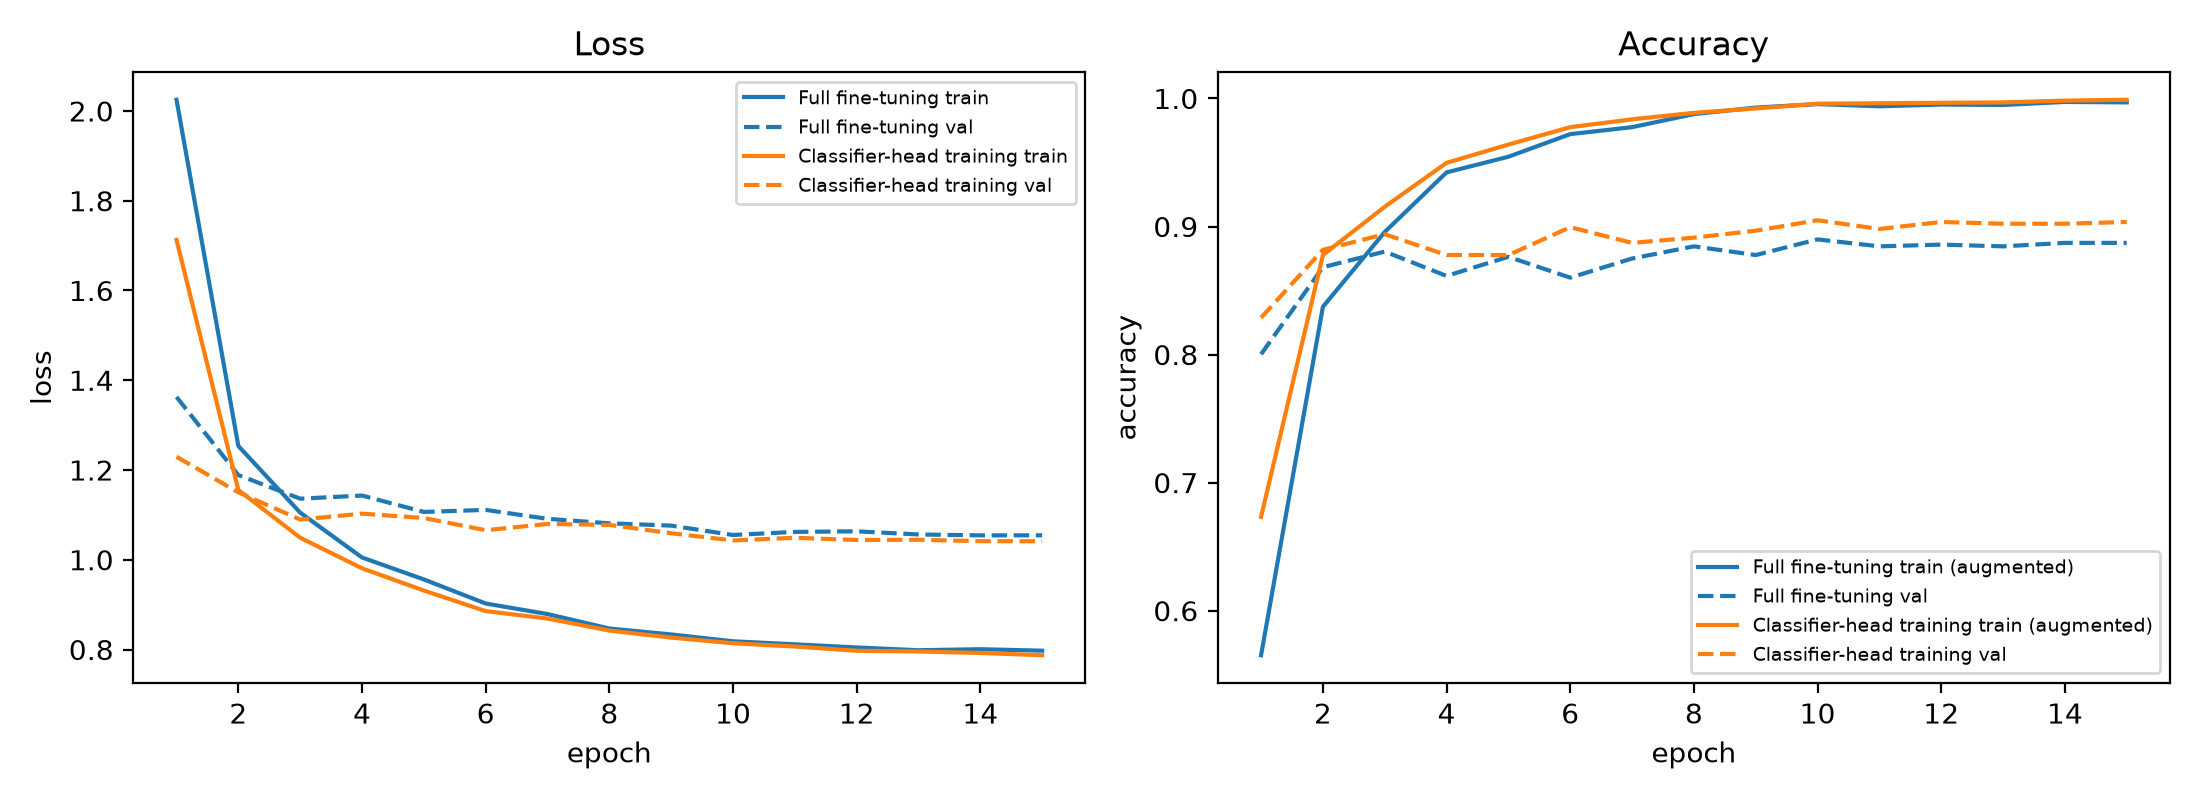
\includegraphics[width=0.9\textwidth]{learning_curves.png}
\caption{Training (augmented) and validation loss and accuracy for approaches 1 and 2. The
training loss does not go below ${\approx}0.8$ because of label smoothing.}
\label{fig:curves}
\end{figure}

\begin{figure}[p]
\centering
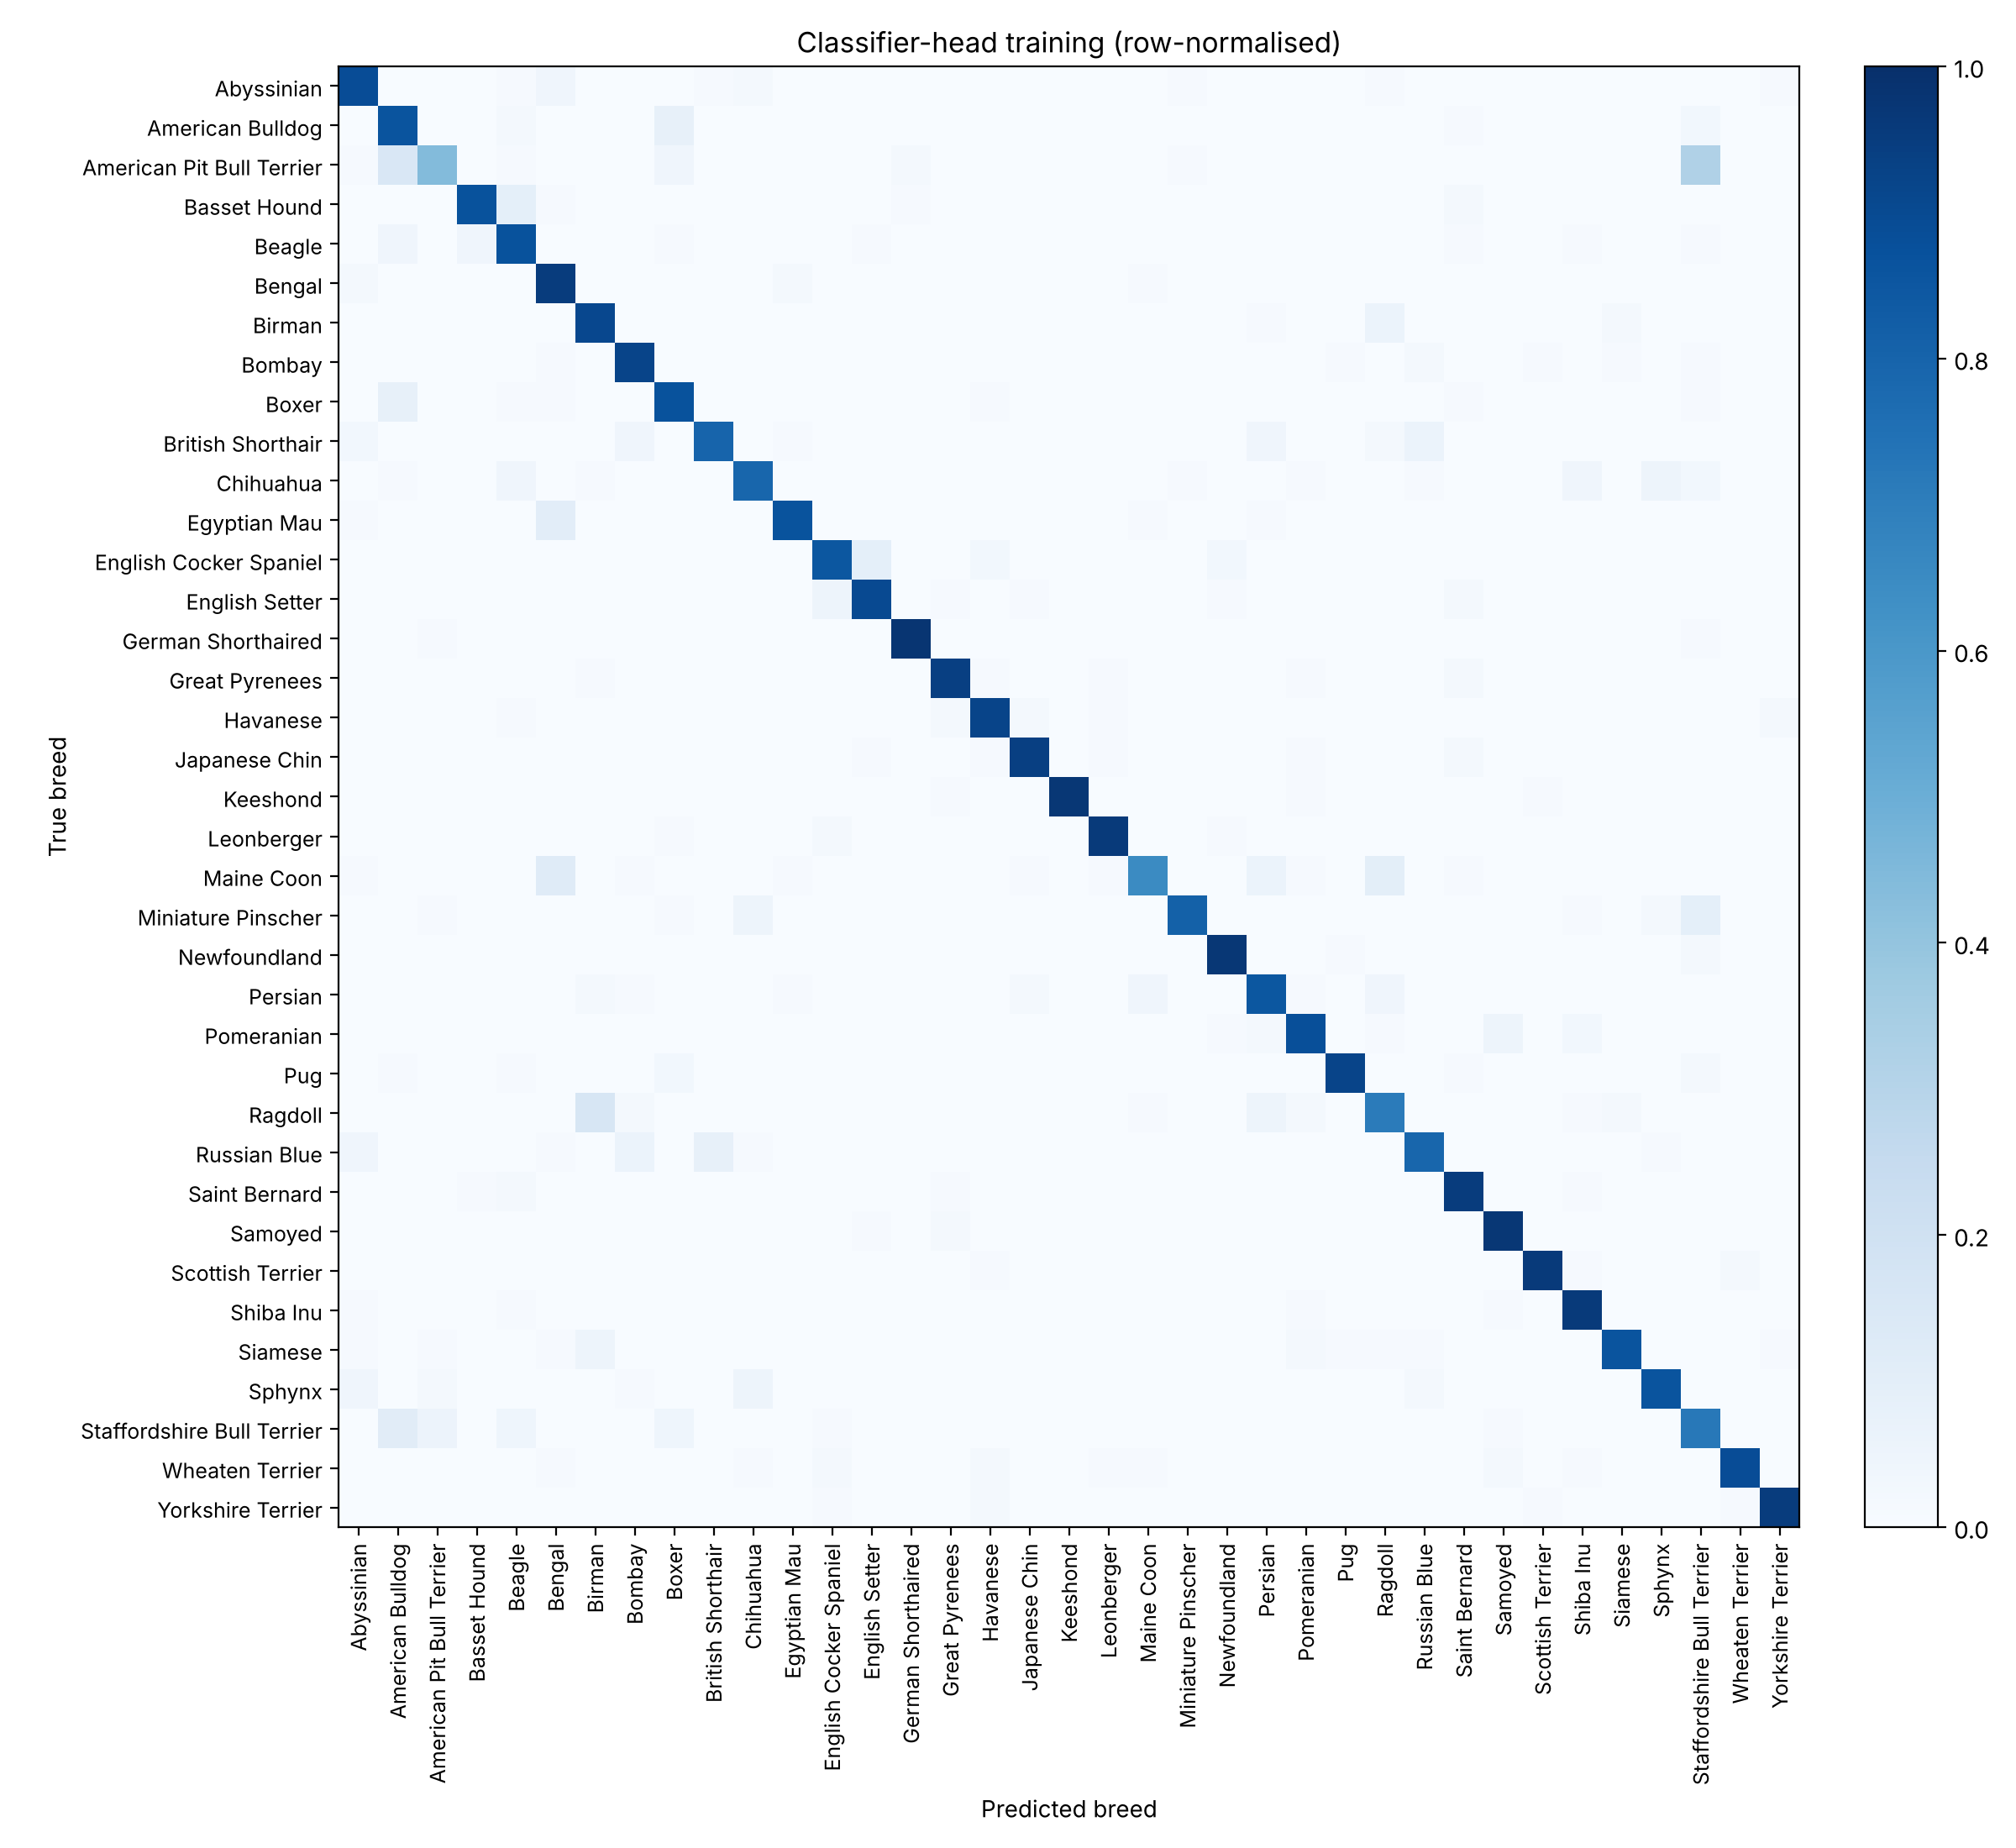
\includegraphics[width=\textwidth]{confusion_head.png}
\caption{Row-normalised test confusion matrix of classifier-head training, the best method
(cell $(i,j)$: fraction of the test images of breed $i$ predicted as breed $j$). The
matrices of the other four methods are in the repository
(\texttt{results/confusion\_*.png}); their most frequent confusions are listed in
\texttt{results/top\_confusions.csv}.}
\label{fig:cm}
\end{figure}

\begin{figure}[tb]
\centering
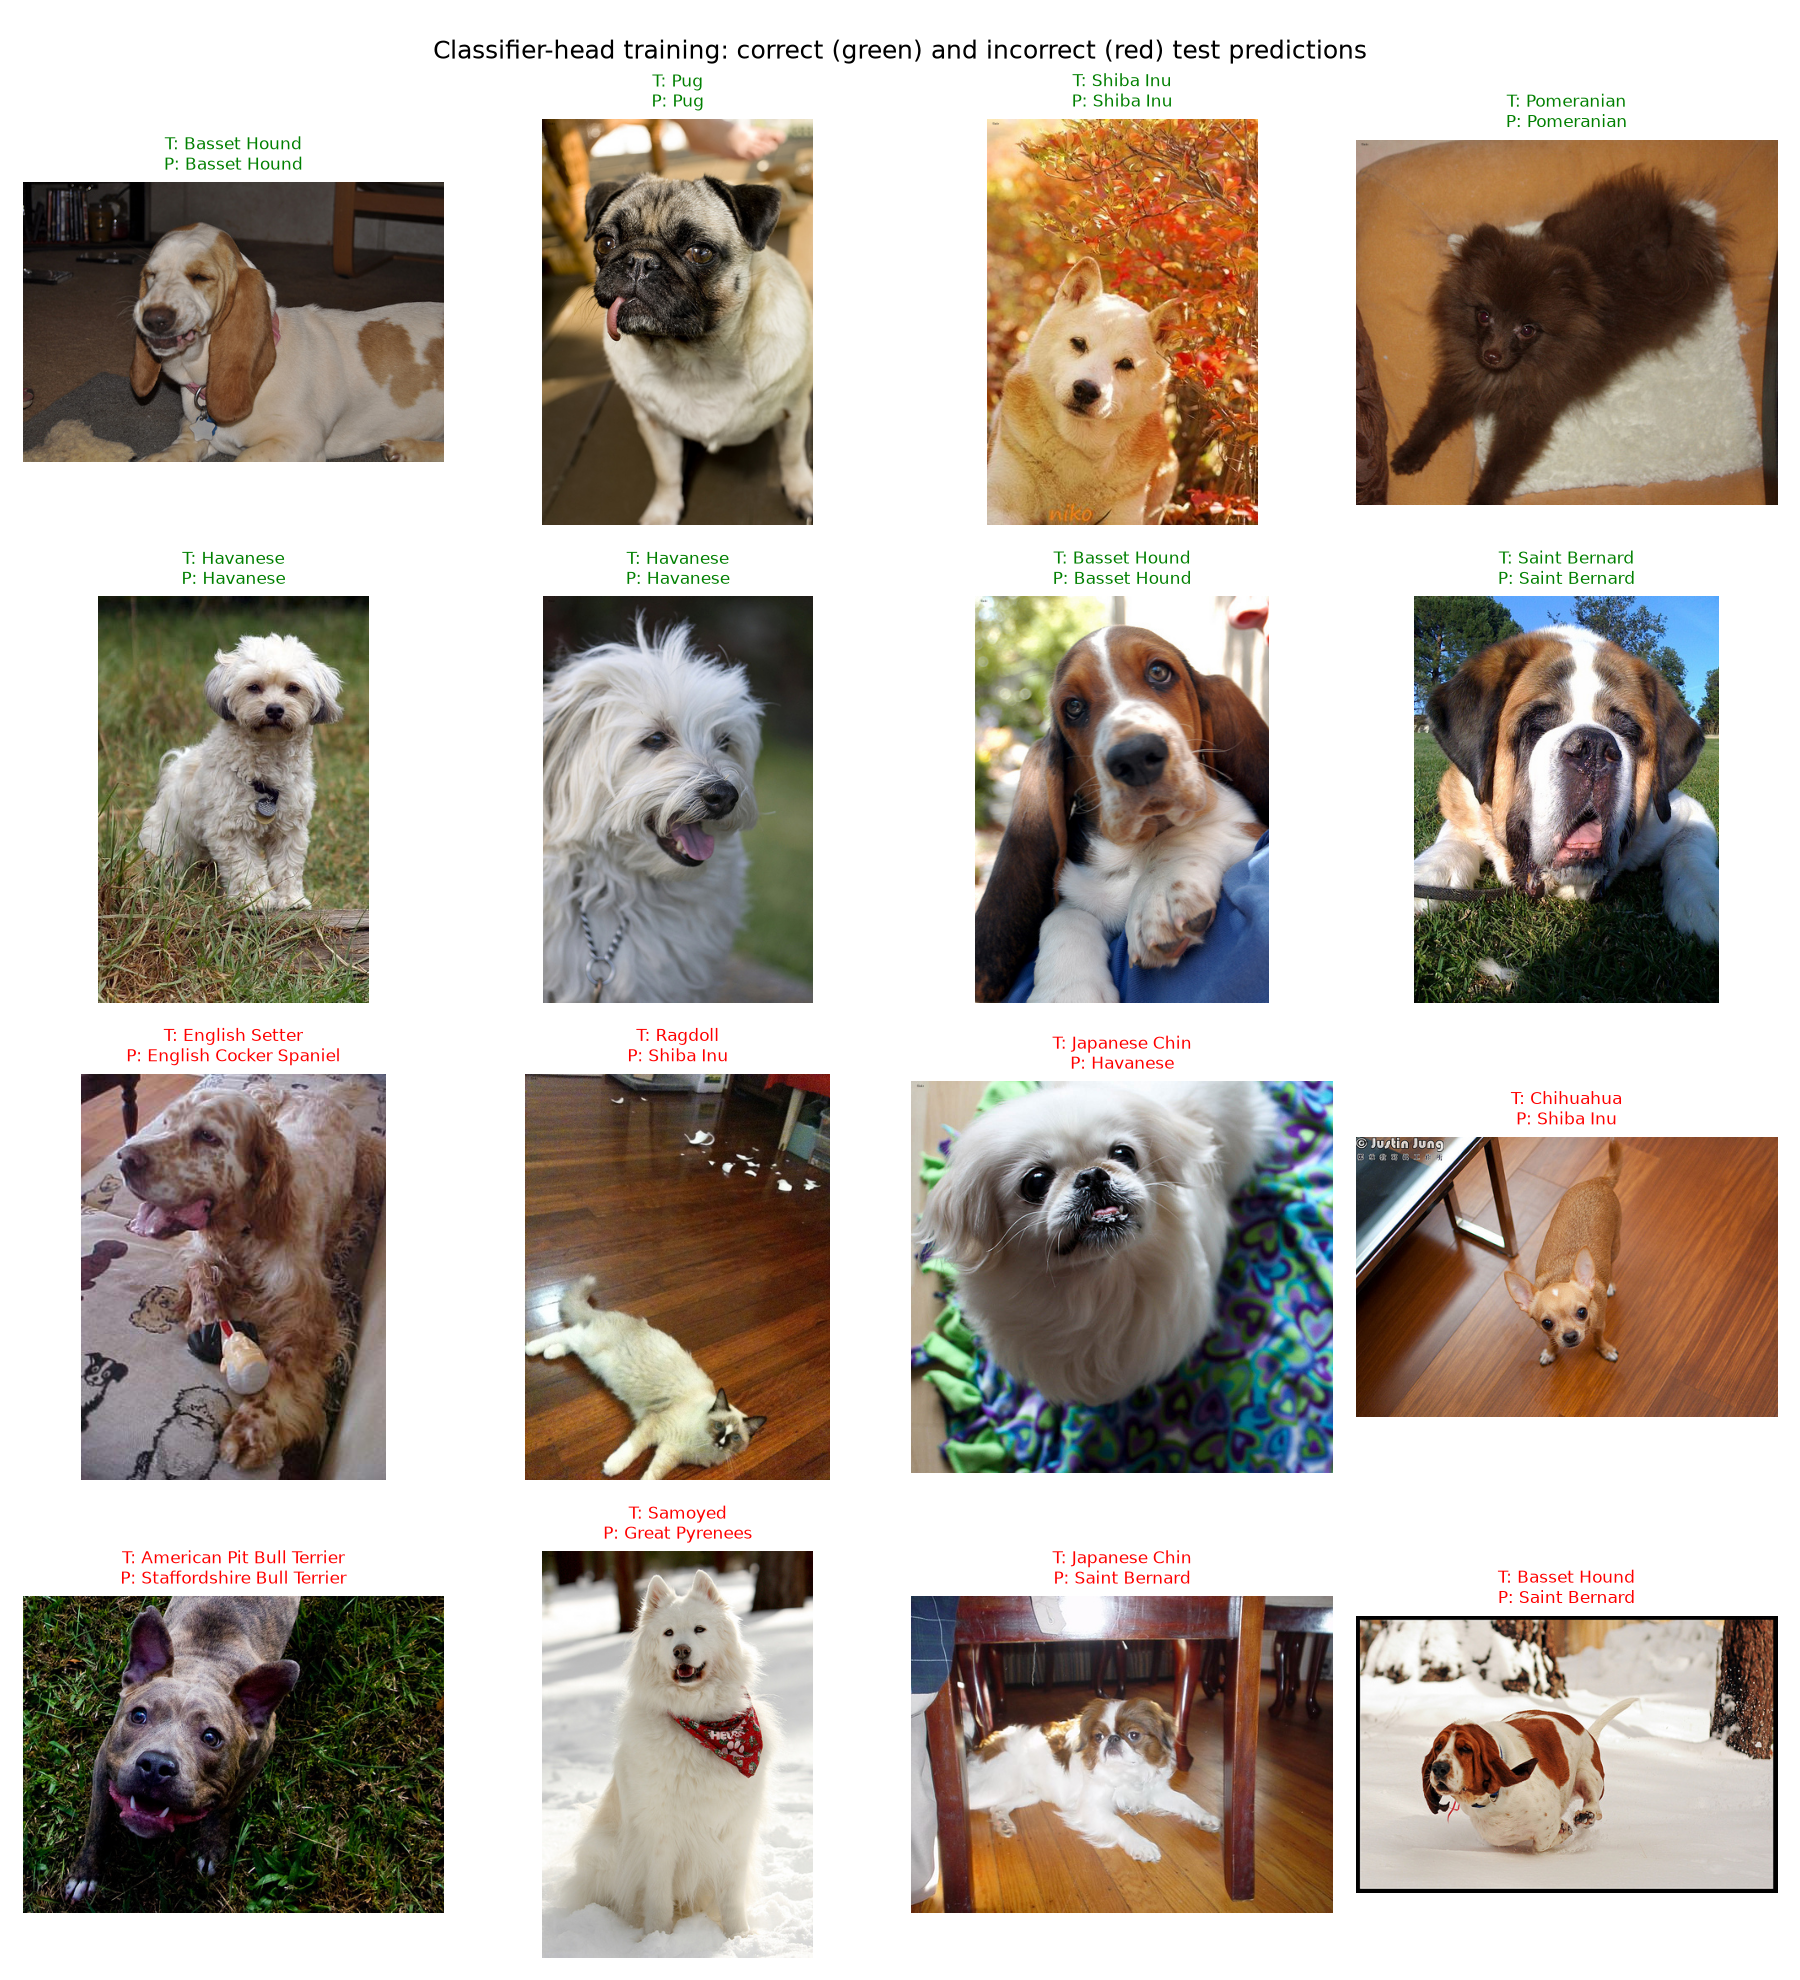
\includegraphics[width=0.56\textwidth]{examples_head.png}
\caption{Randomly sampled correct (green) and incorrect (red) test predictions of
classifier-head training (T: true breed, P: predicted breed).}
\label{fig:examples}
\end{figure}

\section{Discussion}
\paragraph{Performance.} All strategies reach 82--87\% accuracy on a 37-way fine-grained
task, with macro-F1 almost equal to accuracy because the classes are balanced. Training only
the classifier head gives the best result. Full fine-tuning, despite 2.5$\times$ more
trainable parameters, is not better than a simple logistic regression on frozen features.
The paired tests show that the 1.4-point gap between head training and full fine-tuning is
not due to the sampling of the test images. McNemar's test, however, does not account for the
variability due to the random seed (initialisation, augmentation, batch order), so we repeated
approaches 1--2 with two further seeds (1 and 2; \texttt{results/seeds\_summary.csv}). Over the
three seeds, head training reaches $86.9\pm0.2\%$ test accuracy (mean $\pm$ standard deviation)
and full fine-tuning $85.9\pm0.3\%$; head training is better for every seed, by $1.0\pm0.4$
points. The ranking is therefore stable, although three seeds give only a rough estimate of the
size of the gap. Differences smaller than about one point between single runs (e.g.\ full
fine-tuning vs.\ Logistic Regression) should not be considered meaningful.

\paragraph{Overfitting and generalisation.} Every method fits the training set almost
perfectly (98.8--100\%), while test accuracy is 13--17 points lower
(Table~\ref{tab:results}). For approaches 1--2, Fig.~\ref{fig:curves} shows that validation
accuracy plateaus after about 3 epochs (0.86--0.90) while training accuracy keeps rising to
${\approx}1$ and validation loss decreases only slightly, so later epochs mostly memorise the 74--80 images
per class. Full fine-tuning has a larger gap (14.2 points) than head training (12.7) and a
lower validation accuracy at every epoch: with so little data, updating 1.56\,M parameters
adds capacity to overfit but no useful information. The pre-trained features are already
highly discriminative, which we attribute to the similarity between the pre-training and target
domains: ImageNet-1K contains over a hundred dog-breed classes and several domestic cat
classes. Consistently, dog breeds are recognised better than cat breeds by every method
(mean per-class F1 0.88 vs.\ 0.84 for head training, 0.87 vs.\ 0.82 for Logistic Regression),
and full fine-tuning has the smallest cat--dog gap (0.86 vs.\ 0.83), the only setting where the
backbone can adapt to the less represented domain. Among the traditional classifiers, the
Random Forest and the Linear SVM overfit most (train 1.00 and 0.999, gap 17.4 and 16.6
points); the strongly regularised Logistic Regression ($C=0.01$) generalises best.

\paragraph{Computational cost.} Full fine-tuning is the most expensive: gradients must be
propagated through all convolutional layers, so after the first epoch an epoch takes 5.1\,s
vs.\ 1.4\,s for head training (3.6$\times$). The totals in Table~\ref{tab:results}
under-estimate this difference, because each run has a fixed start-up cost of about 20\,s
(spawning the data-loading workers, MPS warm-up, first read of the images from disk): the
first epoch takes 28.2\,s and 22.4\,s respectively. The same overhead dominates feature
extraction, which takes about 42--45\,s for both the validation (736) and test (3{,}669)
sets. Approach 3 needs a single forward pass per image; fitting Logistic Regression then
takes 0.1\,s, so it is the cheapest method to retrain or tune, and it stores only 21\,k
classifier weights on top of the shared backbone. All costs are small in absolute terms
because MobileNetV3-Small is a mobile architecture and the dataset is small.

\paragraph{Error analysis.} Errors are dominated by visually similar breeds of the same
species: 85--90\% of the misclassifications predict a breed of the correct species. The most
frequent confusions are the same for all methods (Fig.~\ref{fig:cm},
\texttt{results/top\_confusions.csv}): American Pit Bull Terrier $\to$ Staffordshire Bull
Terrier (32\% of the Pit Bull test images for head training), Pit Bull $\to$ American
Bulldog, Ragdoll $\leftrightarrow$ Birman, Maine Coon $\to$ Bengal/Ragdoll, Russian Blue
$\to$ British Shorthair and Chihuahua $\to$ Shiba Inu. The lowest per-class F1 scores are
those of the two bull-terrier breeds (0.57 and 0.62 for head training), followed by Ragdoll
(0.72) and Maine Coon (0.75); distinctive breeds such as Keeshond, German Shorthaired and
Newfoundland exceed 0.95. Some of these pairs are hard to separate even for humans and differ
mostly in standards of size or coat pattern that a single photo may not show. The examples in
Fig.~\ref{fig:examples} also suggest a reliance on context and pose: a Basset Hound running in the snow is predicted as Saint Bernard (a breed often photographed
in snow), a Japanese Chin with a similar white-and-brown coat pattern is also predicted as Saint
Bernard, a Samoyed in the snow as Great Pyrenees, and a Ragdoll lying on a wooden floor is predicted as a Shiba
Inu, one of the rare cross-species errors.

\paragraph{Limitations.} (i) The effect of the random seed was measured with only three seeds
for approaches 1--2; Table~\ref{tab:results} and all figures use the seed-42 runs. (ii) For approaches 1--2 only the checkpoint was selected on the
validation set; learning rates, augmentation and number of epochs were fixed a priori, so
full fine-tuning in particular might improve with a lower backbone learning rate or partial
unfreezing. (iii) The validation set has only 19--20 images per class, so model selection is
itself noisy (validation and test accuracies differ by 2--4 points). (iv) Timings were
measured on one machine and include start-up overheads. (v) Results are for a single, small
architecture; larger backbones might benefit more from fine-tuning.

\section{Conclusion}
On Oxford-IIIT Pet, the ImageNet features of MobileNetV3-Small transfer very well: training
only the classifier head achieves the best test accuracy (87.0\%; $86.9\pm0.2\%$ over three seeds) and macro-F1 (0.869) at less
than half the cost of full fine-tuning, and a logistic regression on frozen features matches full
fine-tuning (85.7\% vs.\ 85.6\%) with a classifier that trains in a fraction of a second. With
${\approx}80$ images per class, the extra flexibility of full fine-tuning mainly increases
overfitting. The remaining errors concentrate on a few pairs of visually similar breeds.

\begin{thebibliography}{9}
\bibitem{pets} O.~M. Parkhi, A.~Vedaldi, A.~Zisserman, C.~V. Jawahar.
\newblock Cats and dogs. \newblock In \emph{CVPR}, 2012.
\bibitem{mobilenetv3} A.~Howard et~al.
\newblock Searching for MobileNetV3. \newblock In \emph{ICCV}, 2019.
\bibitem{imagenet} O.~Russakovsky et~al.
\newblock ImageNet large scale visual recognition challenge.
\newblock \emph{International Journal of Computer Vision}, 115(3):211--252, 2015.
\bibitem{pytorch} A.~Paszke et~al.
\newblock PyTorch: an imperative style, high-performance deep learning library.
\newblock In \emph{NeurIPS}, 2019.
\bibitem{sklearn} F.~Pedregosa et~al.
\newblock Scikit-learn: machine learning in Python.
\newblock \emph{Journal of Machine Learning Research}, 12:2825--2830, 2011.
\end{thebibliography}

\end{document}
